\subsection{ISO/IEC 12207}
ISO/IEC 12207 è uno standard utilizzato per misurare la qualità dei processi\ap{G}. Questa normativa è suddivisa in 3 parti
ed ognuna contiene dei sotto processi\ap{G} e delle attività. Il tutto è riportato in seguito. 

\begin{figure}[h]
    \centering
    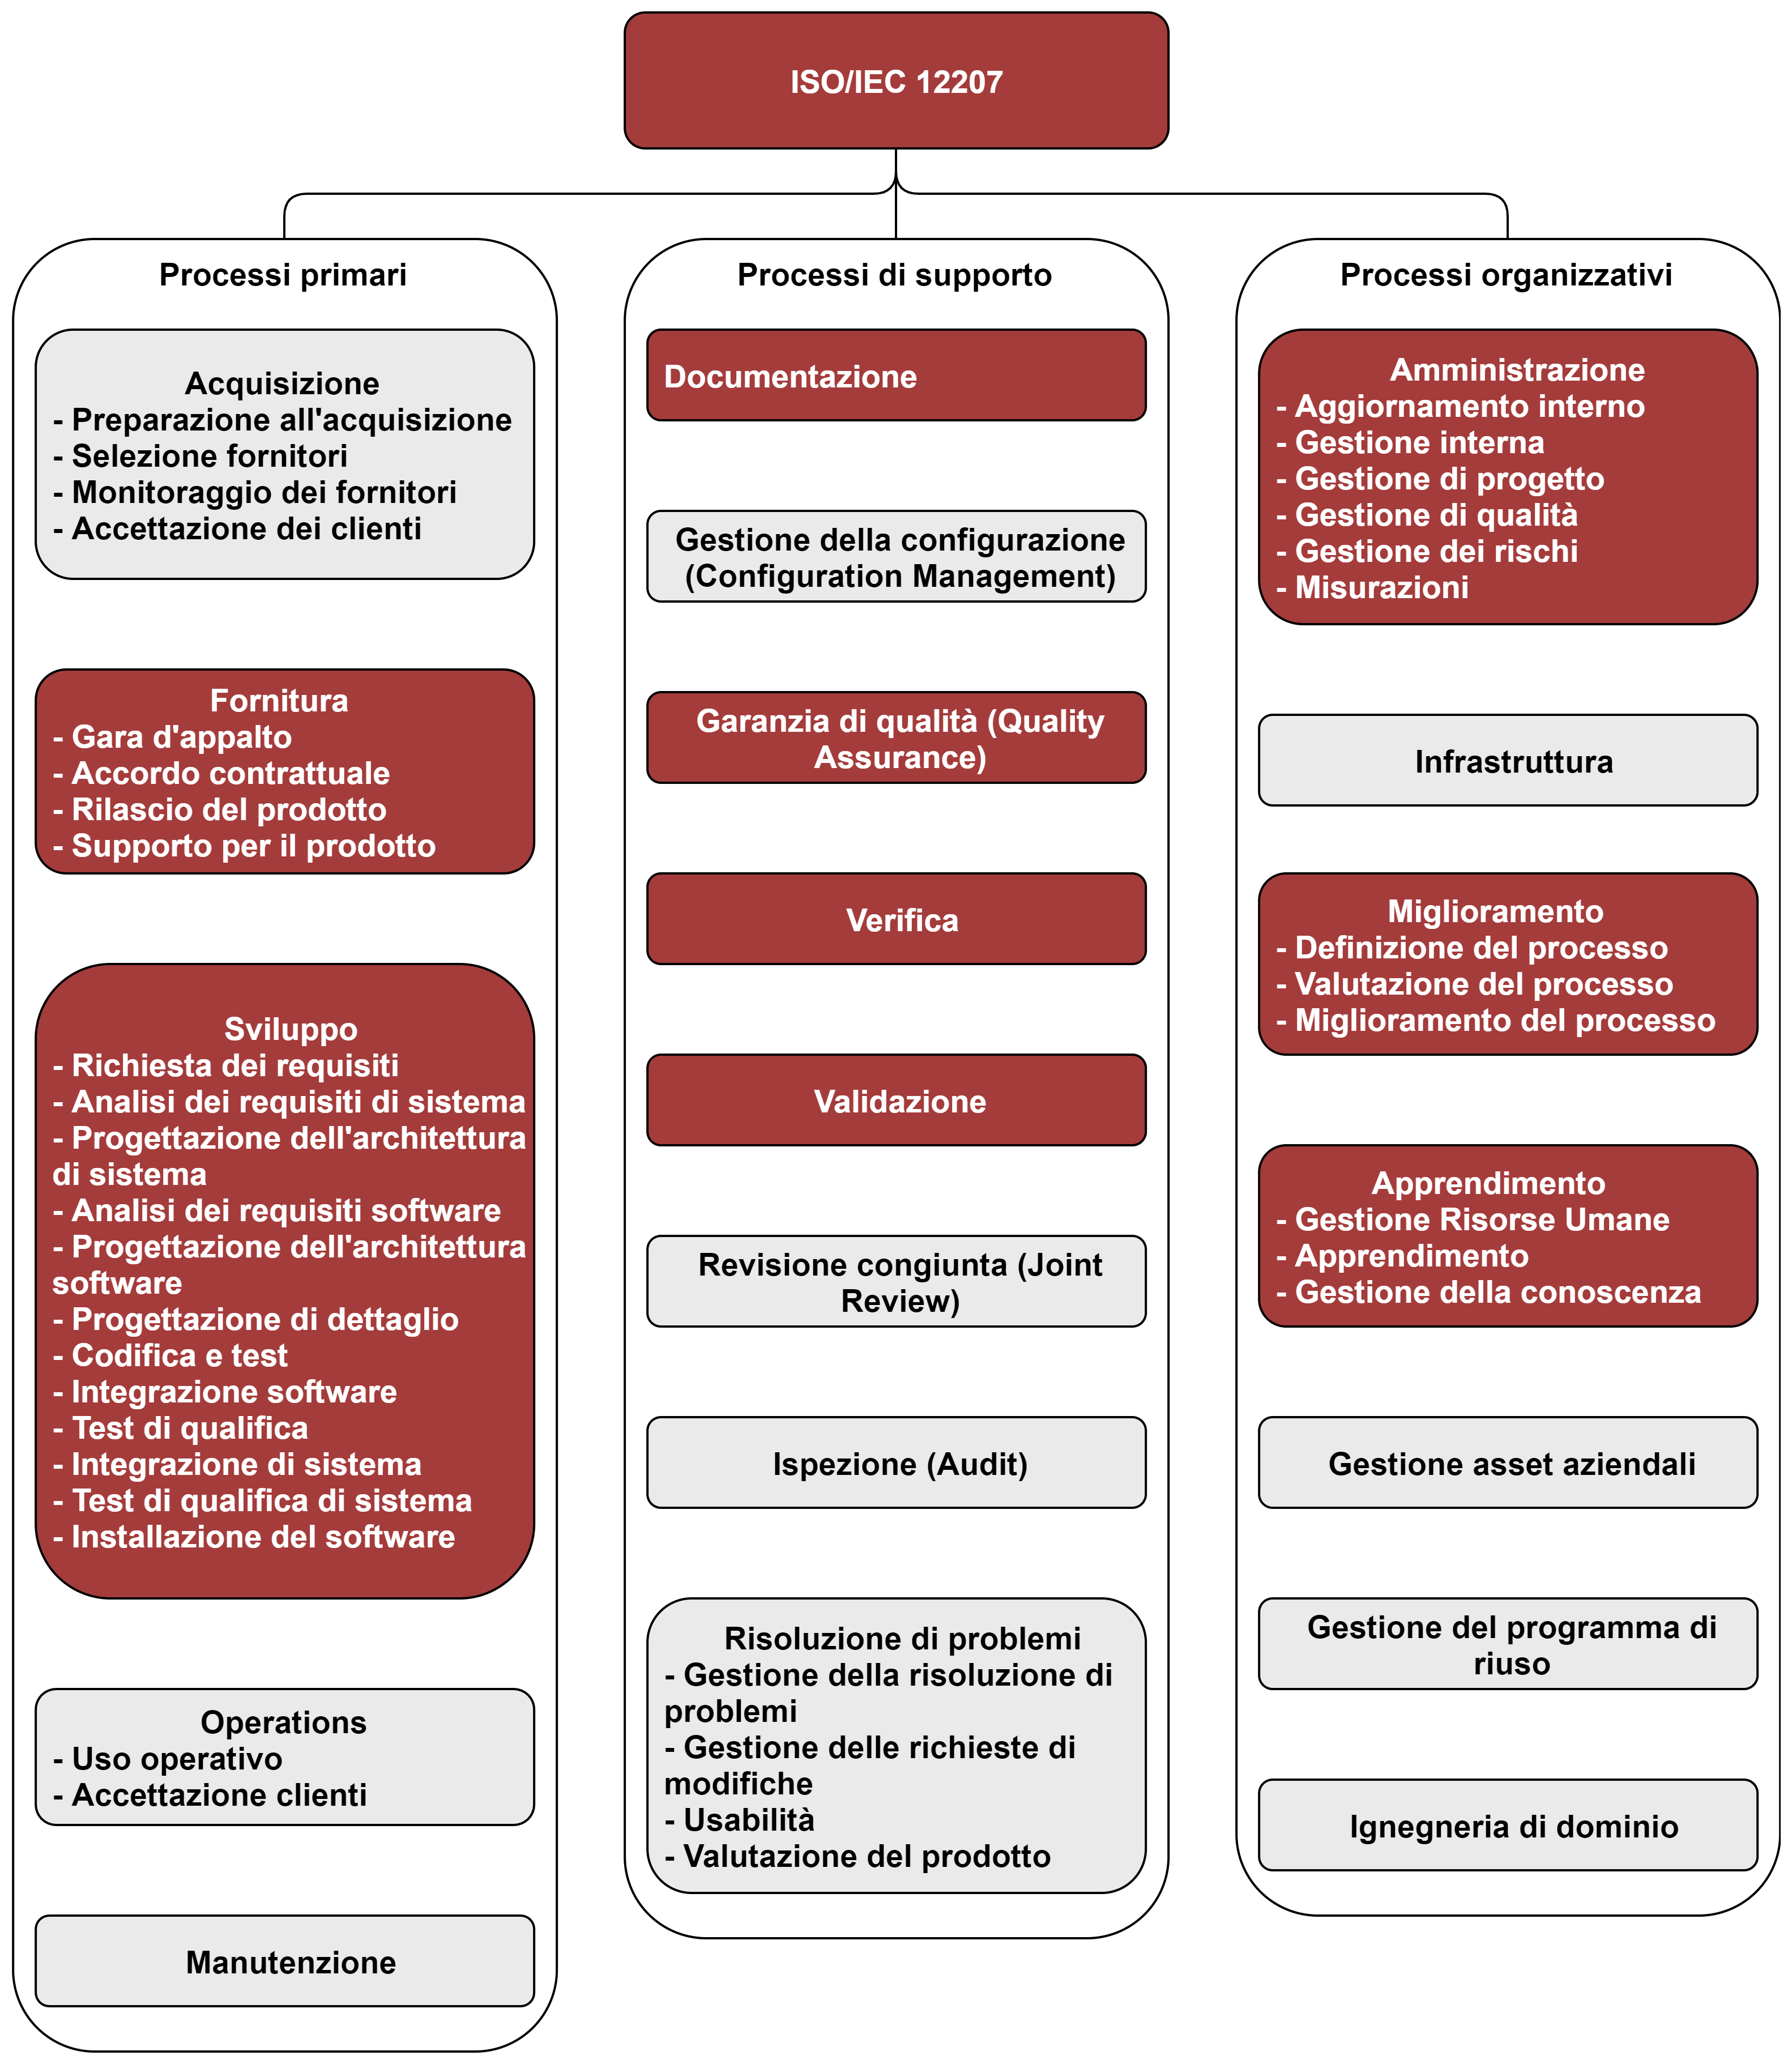
\includegraphics[scale=0.53]{sezioni/Immagini/IsoIec12207.png}
    \caption{Schema dello standard ISO/IEC 12207. In rosso sono indicati i processi e le relative attività di interesse per il progetto.}
\end{figure}

\subsubsection{Processi primari}
Sono i processi\ap{G} e le attività che fanno parte dello sviluppo del software e hanno lo scopo di soddisfare tutti i requisiti concordati con il cliente.

\paragraph{Sviluppo}
Il processo\ap{G} ha lo scopo di sviluppare un prodotto software, o un sistema basato sul software, che indirizzi le esigenze del cliente. \\
I risultati delle valutazioni dei processi\ap{G} devono essere documentati.
\begin{itemize}
    \item \textbf{Analisi dei requisiti:} \\
    Lo sviluppatore deve valutare i requisiti software in base ai criteri elencati di seguito:
        \begin{itemize}
            \item Tracciabilità dei requisiti di sistema e progettazione del sistema;
            \item Coerenza esterna con i requisiti di sistema;
            \item Coerenza interna;
            \item Testabilità\ap{G};
            \item Fattibilità della progettazione del software;
            \item Fattibilità di funzionamento e manutenzione.
        \end{itemize}
    \item \textbf{Pianificazione di dettaglio:} \\
    Lo sviluppatore deve sviluppare un progetto dettagliato per ciascun componente software. I componenti del software 
    devono essere perfezionati in livelli inferiori contenenti unità software che possono essere codificati, compilati 
    e testati. È necessario garantire che tutti i requisiti software siano assegnati dai componenti software 
    alle unità software.
    
    \item \textbf{Codifica:} \\
    Lo sviluppatore deve valutare il codice del software e i risultati dei test considerando i criteri elencati sotto:
    \begin{itemize}
        \item Tracciabilità ai requisiti e alla progettazione dell'articolo software;
        \item Coerenza esterna con i requisiti e il design dell'articolo software;
        \item Coerenza interna tra i requisiti dell'unità;
        \item Testare la copertura delle unità;
        \item Adeguatezza dei metodi e delle norme di codifica utilizzati;
        \item Fattibilità dell'integrazione e dei test del software;
        \item Fattibilità di funzionamento e manutenzione.   
    \end{itemize}
\end{itemize}

\subsubsection{Processi di supporto}
Sono i processi\ap{G} e le attività che aiutano gli altri processi\ap{G} nel raggiungimento del successo e nella qualità del progetto.

\paragraph{Documentazione}
Il processo\ap{G} di "Gestione della documentazione" garantisce lo sviluppo e la manutenzione delle informazioni prodotte e registrate relativamente al prodotto software. \\ \\
\textbf{Implementazione:} \\ 
Identifica i documenti da produrre durante il ciclo di vita del prodotto software;
deve essere sviluppato, documentato e implementato. La documentazione dovrà prevedere i seguenti punti: 
\begin{itemize}
    \item Titolo o nome;
    \item Scopo;
    \item Pubblico previsto;
    \item Procedure e responsabilità per input, sviluppo, revisione, modifica, approvazione, produzione, stoccaggio, distribuzione, manutenzione e gestione della configurazione;
    \item Programma per le versioni intermedie e finali.
\end{itemize}

\paragraph{Garanzia di qualità}
Il processo\ap{G} di "Assicurazione qualità" ha lo scopo di assicurare che tutti i prodotti di fase (work product) siano conformi con i piani e gli standard definiti.
\paragraph{Verifica}
Il processo\ap{G} di verifica ha lo scopo di confermare che ciascun work product o servizio realizzato da un processo\ap{G} soddisfi i requisiti specificati. 
Il processo\ap{G} di verifica deve essere integrato nei processi\ap{G} di Sviluppo, Fornitura e Manutenzione. Se la verifica viene eseguita da terzi, questa viene definita come "Processo\ap{G} di verifica indipendente".
\\
Il processo\ap{G} deve essere verificato considerando i criteri elencati di seguito:
\begin{itemize}
    \item I requisiti di pianificazione del progetto sono adeguati e tempestivi;
    \item I processi\ap{G} selezionati per il progetto sono adeguati, implementati, eseguiti come previsto, e conformi al contratto.
    \item Gli standard, le procedure e gli ambienti per i processi\ap{G} del progetto sono adeguati.
    \item Il progetto è composto da personale qualificato capace di soddisfare le richieste del contratto.
\end{itemize}

\subsubsection{Processi organizzativi}
Sono i processi\ap{G} e le attività che coprono gli aspetti organizzativi e di gestione delle risorse.

\paragraph{Gestione}
Il processo\ap{G} di gestione garantisce lo sviluppo e la manutenzione delle informazioni prodotte e registrate relativamente 
al prodotto software. L'amministratore prepara i piani per l'esecuzione del processo\ap{G}.
I piani associati all'esecuzione del processo\ap{G} devono contenere descrizioni: delle attività, dei compiti associati e
identificazioni dei prodotti software che verranno forniti. Questi piani devono rispettare i seguenti punti:
\begin{itemize}
    \item Programmi per il completamento tempestivo dei compiti;
    \item Risorse adeguate necessarie per eseguire i compiti;
    \item Assegnazione di compiti;
    \item Assegnazione di responsabilità;
    \item Quantificazione dei rischi associati ai compiti o al processo\ap{G} stesso;
    \item Misure di controllo della qualità da applicare durante l'intero processo\ap{G};
    \item Costi associati all'esecuzione del processo\ap{G};
    \item Fornitura di ambiente e infrastruttura.
\end{itemize}
